% ----------------------------------------------------------
% Introdução
% ----------------------------------------------------------
\chapter{Introdução}\label{sec:Introdução}

A tecnologia da informação está presente em todos os segmentos da sociedade, abrangendo desde o lazer até diversas atividades e serviços. Dessa forma, sua utilização proporciona ganhos significativos em conhecimento, reduz o tempo necessário para encontrar soluções e esclarece quais passos e produtos podem resolver problemas específicos. Assim, aqueles que utilizam a tecnologia da informação ganham notoriedade por sua eficiência e eficácia \mbox{\cite{a:gestao_inovacao_2024}.}

 Assim é essencial que as empresas estejam sempre aprimorando suas atividades para aumentar a produtividade e se destacar no mercado. Nesse contexto, a implementação de Sistemas de Informação (SI), desempenha um papel fundamental, permitindo a análise rápida de cenários e ajudando a empresa a otimizar suas operações mais relevantes \mbox{\cite{a:tecnologia_empresa_2024}.}

De fato, o setor de administração e gestão deve possuir um profundo conhecimento e compreensão das informações geradas pelas atividades do negócio. Não há espaço para ``achismos'' ou uma condução amadora da empresa, pois, se os responsáveis pela gestão não prestarem a devida atenção nas etapas e ciclos que compõem seu ramo de atividade, a probabilidade de perder oportunidades e até mesmo enfrentar a falência aumenta consideravelmente \mbox{\cite{b:administracao_gestao_2024}}. Ao analisar o cenário, é possível neutralizar ou minimizar potenciais riscos. Além disso, um obstáculo pode ser transformado em uma oportunidade quando identificado com antecedência, graças a uma gestão eficaz que utiliza a tecnologia da informação e demonstra interesse em inovar \mbox{\cite{a:gestao_inovacao_2024}}.

A empresa V Tornos é uma microempresa de capital limitado com mais de cinco anos de experiência no mercado, especializada na manutenção de equipamentos agrícola e pecuária. Sendo um negócio familiar, ela desenvolve suas atividades documentais utilizando blocos de notas e planilhas de Excel para organizar e registrar suas operações. Dessa forma, a implementação de um sistema informatizado de gestão documental para suas operações e administração se torna crucial para possibilitar futuras expansões e otimizações no segmento em que atua.

Este projeto tem como objetivo desenvolver um sistema de suporte a orçamentos e serviços que gere informações sobre quais equipamentos apresentam o maior número de reparos. Dessa forma, a implementação de um software tem como objetivo inovar a empresa V Tornos, atualizando a documentação das operações para enfrentar os desafios e aproveitar as oportunidades no dinâmico segmento de manutenção em usinagem. Neste contexto, é fundamental desenvolver a capacidade de explorar novas oportunidades, integrar conhecimentos, utilizar recursos internos e externos, e estar em constante aperfeiçoamento e adaptação para às mudanças e incertezas do mercado.


Este trabalho está organizado da seguinte forma: a Seção \ref{sec:justificativa} apresenta a justificativa; a Seção \ref{sec:problema} especifica o cenário onde o software implementará as melhorias; a Seção \ref{sec:objetivo} delineia as intervenções da aplicação; a Seção \ref{sec:fundamentacao} aborda a história da industrialização, tipos de manutenção, conceitos de usinagem e breve contextualização sobre sistemas web; a Seção \ref{sec:metodologia} apresenta o modelo de caso de uso e o diagrama de Entidade Relacionamento com as tabelas do banco de dados; e, por fim, a última seção apresenta o cronograma de desenvolvimento de cada atividade.

\section{Justificativa}\label{sec:Justificativa}

A empresa V. Tornos é uma microempresa que oferece serviços no setor de maquinário para agricultura e pecuária. Suas atividades envolvem usinagem para reparos parciais ou fabricação de peças novas em situações de avarias graves que requerem substituição. De modo que as peças são reparadas ou fabricadas artesanalmente, seguindo medidas precisas para atender às dimensões da máquina e garantir o funcionamento correto das partes do equipamento. Adicionalmente, os clientes costumam solicitar serviços de adaptação para melhorar o desempenho ou prolongar a vida útil das peças sujeitas ao desgaste devido ao uso constante.

A empresa, conforme ilustrado na Figura \ref{fig:diagrama_VTornos}, adota um processo estruturado para realizar a manutenção de peças e equipamentos. O processo inicia com uma inspeção, que inclui a desmontagem dos componentes para identificar avarias ou desgastes. Em seguida, uma análise dos componentes é conduzida. Baseado nos resultados, é feito uma classificação para determinar o grau de desgaste e as causas das falhas, criando uma documentação apropriada para futuras referências. Com essas informações, um plano de manutenção é desenvolvido, detalhando as ações necessárias, como reparos ou substituições, e essa proposta é comunicada ao cliente. A manutenção é então executada após a aprovação, ou o equipamento é devolvido caso o cliente opte por não realizar a reparação com a V Tornos.

\begin{figure}[htb!]
    \centering
    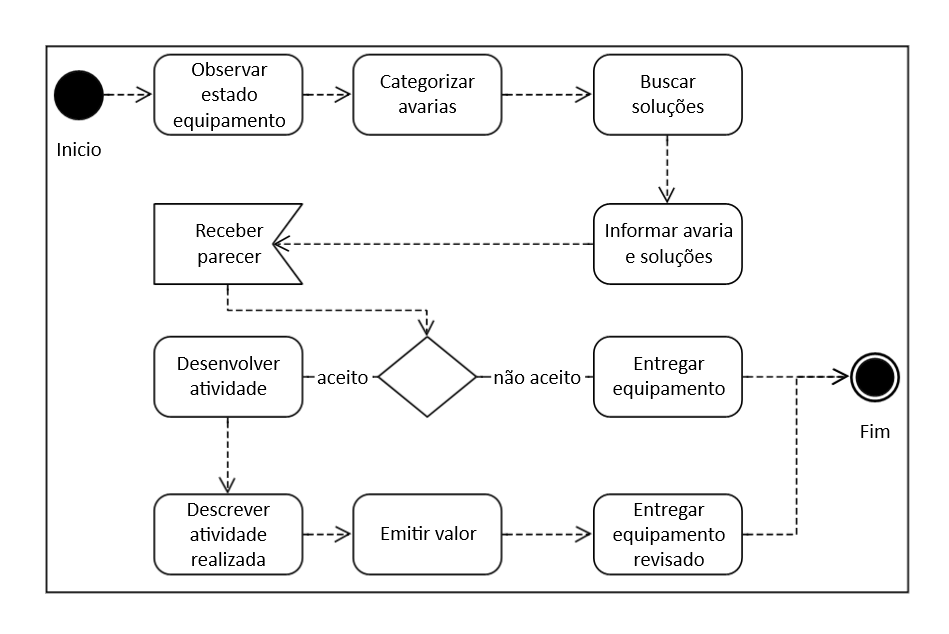
\includegraphics[width=.75\linewidth]{figs/diagrama_atividade_VTornos.png}
    \caption{Passos da V Tornos para realizar manutenção de peça ou equipamento}
    \label{fig:diagrama_VTornos}
\end{figure}

Dessa forma, a empresa tem como objetivo central a manutenção, pois desenvolve peças para situações específicas conforme os parâmetros dos maquinários já com tempo de uso. Isso a diferencia de uma empresa de produção industrial, onde existe um modelo computacional já pronto para uso e um cronograma mensal definindo quais peças serão produzidas em tornos automatizados, sem produção de peças fora do padrão estabelecido.

A proposta para este trabalho inclui a implementação de um sistema de orçamentos para a V. Tornos, levando em consideração os requisitos para a prestação de serviços. É fundamental manter um equilíbrio entre as operações e inovações para garantir uma administração saudável, de forma a aproveitar as oportunidades do mercado. O sistema permitirá visualizar quais atividades estão sendo mais desenvolvidas, auxiliando na tomada de decisões e na identificação de áreas de foco para o crescimento da empresa.

\section{Objetivos}

As finalidades do trabalho são pontuadas a partir das seguintes questões, conforme descrito nas subseções geral e específicos.

\subsection{Geral}\label{sec:objGeral}

Desenvolver sistema de gestão de orçamento e serviços para melhoria operacional e administrativa da empresa V. Tornos.

\subsection{Objetivos Específicos}\label{sec:objEspc}

\begin{itemize}
   \item Melhorar a gestão de dados dos cliente e respetivas inscrições municipais e estaduais;
   \item Manter registros de serviços já prestados para futuras consultas;
   \item Facilitar o controle de insumos ofertados para os clientes;
   \item  Gerar relatórios e dashboards específicos para tomada de decisões empresariais.
\end{itemize}